\documentclass[11pt,a4paper]{book}
\textwidth 170 mm
\textheight 250 mm
\topmargin -15 mm
\oddsidemargin -5 mm
\evensidemargin -5 mm

\newcounter{ProblemNo}
\setcounter{ProblemNo}{0}
\def\tempID{0}
%\def\UndAns{} %% <-------------- Uncomment in final version!!
\def\UndAns{\underline}
\def\UndAns{\underline}
\newcommand{\ZOdg}[1]{}
\def\text{}
%\def\dfrac{\displaystyle\frac}

\usepackage{amsfonts,amssymb,amsmath}
\usepackage{graphicx}
\DeclareGraphicsExtensions{.pdf,.PDF,.png,.PNG} % prefer pdf to png
\usepackage{etoolbox}
\usepackage{sidepicture}
\newcommand{\problemID}[3]{\def\tempID{#1 (#3)}\ignorespacesafterend}
%\newcommand{\problemID}[3]{\def\tempID{#1}\noindent{\bf #1, #2}\par}
%\newcommand{\problemID}[3]{\def\tempID{#3: \##1}\par}
%\newcommand{\problemRating}[3]{{\bf #1, #2, #3}\par}
%\newcommand{\problemID}[3]{\def\tempID{\# #1}\par}
%\newcommand{\problemRating}[3]{}
%\newcommand{\xProblem}[8]{#1\par (A) #2\quad (B) #3\quad  (C) #4\quad  (D) #5\quad (E) #6\par Correct: #7\bigskip\bigskip\par }

%\usepackage{xcolor}
%\usepackage{everypage}
%\usepackage[absolute]{textpos}
%\usepackage{rotating}
%\AddEverypageHook{\begin{textblock*}{2.5cm}(0.7cm,5cm)\begin{turn}{90}{\color{red}\Huge\sc Solutions included - do not use for contest}\end{turn}\end{textblock*}}

\newcommand{\Problem}[9]
{%\newpage
%\noindent\addtocounter{ProblemNo}{1}{\bf\arabic{ProblemNo}.\hspace{3pt}~}%
\noindent\addtocounter{ProblemNo}{1}{\bf\tempID.\hspace{3pt}~}%
\edef\answer{{#7}}\def\SettingMode{#8}%
\def\VLine{\vrule height14pt width0pt\quad}#1\nopagebreak\vspace{1ex}\newline%
\VLine\expandafter\ifstrequal\answer{A}{\UndAns{(\rlap{\bf A}\phantom{\bf C})}\ZOdg{A}}{(\rlap{\bf A}\phantom{\bf C})}\nolinebreak\hspace{3pt}%
\ifnum\SettingMode=3{#2}\else\rlap{#2}\fi\quad\ifnum\SettingMode=3\newline\VLine\else\hfil\fi%
\expandafter\ifstrequal\answer{B}{\UndAns{(\rlap{\bf B}\phantom{\bf C})}\ZOdg{B}}{(\rlap{\bf B}\phantom{\bf C})}\nolinebreak\hspace{3pt}%
\ifnum\SettingMode=3{#3}\else\rlap{#3}\fi\quad\ifnum\SettingMode=2\newline\VLine\else\ifnum\SettingMode=3\newline\VLine\else\ifnum\SettingMode=6{\phantom{({\bf C})}\quad\hspace{6pt}\hfil\hfil\newline\VLine}\else\hfil\fi\fi\fi%
\expandafter\ifstrequal\answer{C}{\UndAns{(\rlap{\bf C}\phantom{\bf C})}\ZOdg{C}}{({\bf C})}\nolinebreak\hspace{3pt}%
\ifnum\SettingMode=3{#4}\else\rlap{#4}\fi\quad\ifodd\SettingMode\newline\VLine\else\hfil\fi%
\expandafter\ifstrequal\answer{D}{\UndAns{(\rlap{\bf D}\phantom{\bf C})}\ZOdg{D}}{(\rlap{\bf D}\phantom{\bf C})}\nolinebreak\hspace{3pt}%
\ifnum\SettingMode=3{#5}\else\rlap{#5}\fi\quad\ifnum\SettingMode>1\ifnum\SettingMode<6\newline\VLine\else\hfil\fi\else\hfil\fi%
\expandafter\ifstrequal\answer{E}{\UndAns{(\rlap{\bf E}\phantom{\bf C})}\ZOdg{E}}{(\rlap{\bf E}\phantom{\bf C})}\nolinebreak\hspace{3pt}%
\ifnum\SettingMode=3{#6}\else\rlap{#6}\fi\quad\ifnum\SettingMode=1\hfil\phantom{({\bf C})}\fi\hspace{3pt}\hfil\par\vspace{2ex}\par\noindent{\sc Solution: }#9\bigskip}


\def\TheHead{Pre-Ecolier Finalized}
\makeatletter
\def\ps@pKSF{
\def\@oddfoot{\hfill{\rm \thepage}\hfill}\def\@evenfoot{\hfill{\rm \thepage}\hfill}
\def\@oddhead{\hfill{\em \TheHead}\hfill}\def\@evenhead{\hfill{\em \TheHead}\hfill}
}
\makeatother 
\pagestyle{pKSF}

\begin{document}

\noindent{\large\bf Pre-Ecolier}\bigskip

\noindent\fbox{3 points}\bigskip

\problemID{1}{20149}{China}%
\problemRating{P}{3}{G}%
\Problem{Which number is inside the triangle, the square and the circle? 
\newline
\centerline{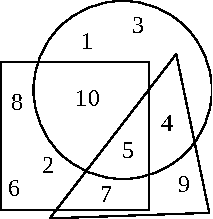
\includegraphics{P01-1}}}
{1}{4}{5}{9}{12}
{C}{0}
{Looking at the picture, number 5 is the only number in all three shapes.}

\problemID{2}{20150}{China}%
\problemRating{P}{3}{G}%
\Problem{Some shapes are printed on 2 pieces of glass. Anna places one on top of the other, without turning either piece.  What does she see?
\newline
\centerline{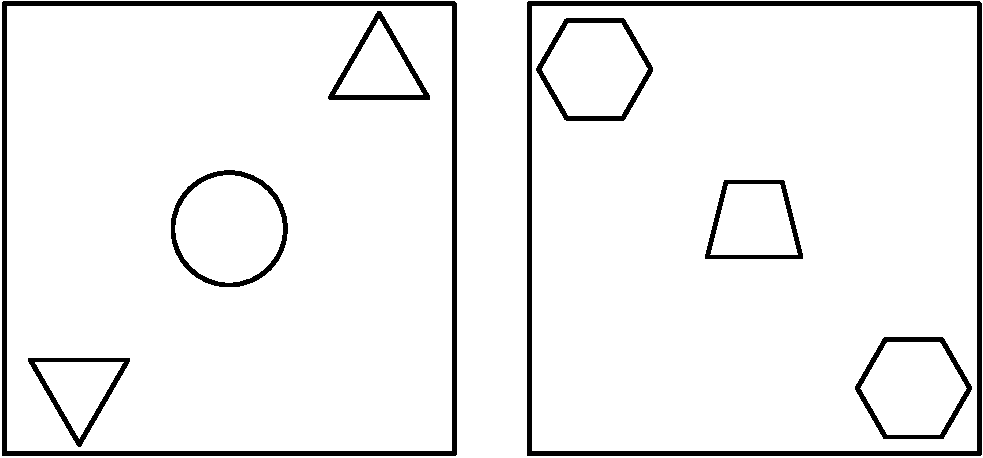
\includegraphics{P02-1}}}
{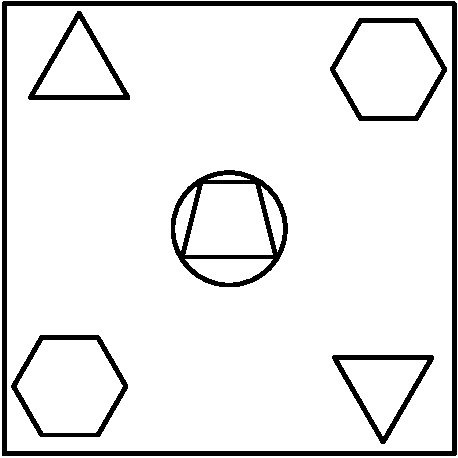
\includegraphics{P02-2}}{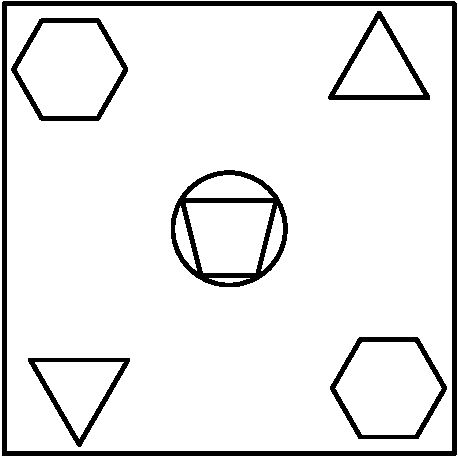
\includegraphics{P02-3}}{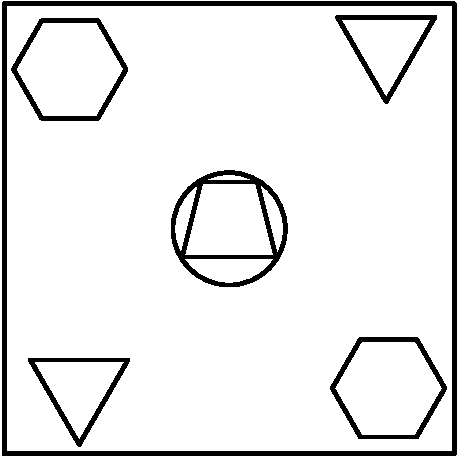
\includegraphics{P02-4}}{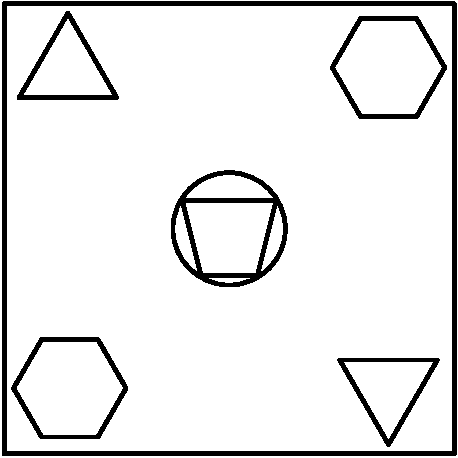
\includegraphics{P02-5}}{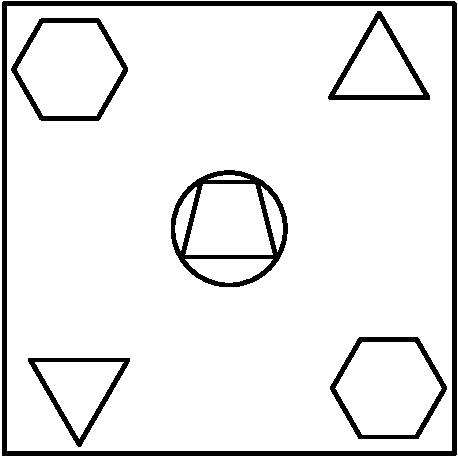
\includegraphics{P02-6}}
{A}{1}
{When the shapes overlap, the hexagons remain in the top left and bottom right corners. Also the triangles remain in the top right and bottom left corners.  This eliminates choices (D) and (E). Next we can eliminate choice (B) because the shape in the centre is inverted. Looking more closely at choice (C), we notice that the triangle in the top right corner is inverted. That leaves us with choice (A).}

\problemID{3}{20151}{Greece}%
\problemRating{P}{3}{G}%
\Problem{The picture shows 4 strange shapes. How many shapes have 3 dots inside?
\newline
\centerline{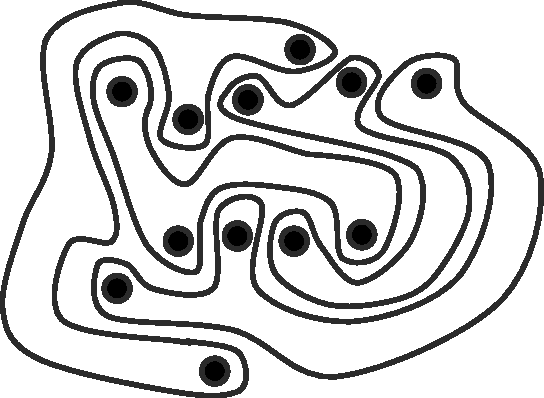
\includegraphics[scale=0.8]{P03-1}}}
{0}{1}{2}{3}{4}
{E}{0}
{By colouring the shapes, they are easier to recognize. Then we can see that all 4 shapes have 3 dots inside.  
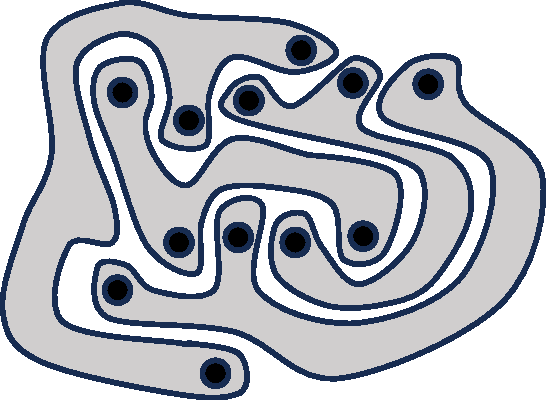
\includegraphics{P03-2}}

\problemID{4}{20152}{Russia}%
\problemRating{P}{3}{G}%
\Problem{Kevin the kangaroo puts a picture on the table.
\newline
\centerline{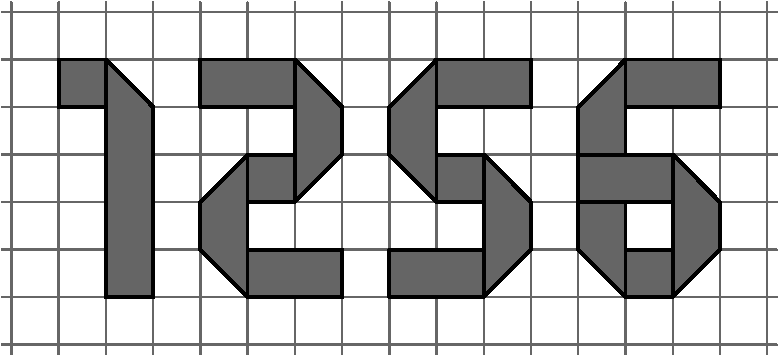
\includegraphics{P04-1}}
\newline
He rotates the picture through a quarter turn, as shown. He then does the same rotation again.
What does Kevin see now?}
{\includegraphics{P04-2}}{\includegraphics{P04-3}}{\includegraphics{P04-4}}{\includegraphics{P04-5}}{\includegraphics{P04-6}}
{C}{0}
{\includegraphics{P04-7}}

\problemID{5}{20153}{Catalonia}%
\problemRating{P}{3}{L}%
\Problem{In the picture, there are 8 different faces. \newline
\centerline{
\includegraphics{P05-1}}
\newline
Each face appears twice, except for one. Which face appears only once?}
{
\includegraphics{P05-2}}{
\includegraphics{P05-3}}{
\includegraphics{P05-4}}{
\includegraphics{P05-5}}{
\includegraphics{P05-6}}
{C}{0}
{After matching all the possible pairs, (C) is the only face that appears just once.}

\problemID{6}{20154}{Malaysia}%
\problemRating{P}{3}{G}%
\Problem{Bruno is making this large triangle using identical small triangular tiles.\newline
\centerline{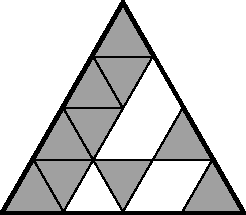
\includegraphics{P06-1}}\newline
How many more tiles does Bruno need to complete the large triangle?}
{3}{4}{5}{6}{7}
{D}{0}
{Bruno needs six identical triangle tiles to complete the picture, as shown.\newline
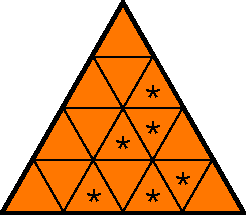
\includegraphics{P06-2}}

\problemID{7}{20155}{Myanmar}%
\problemRating{P}{3}{G}%
\Problem{Each number below is made using a piece of ribbon.\newline
\centerline{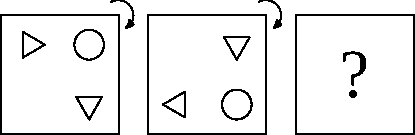
\includegraphics[scale=0.75]{P07-1}}\newline
Which piece of ribbon is the longest?}
{1}{2}{5}{6}{They are all the same length.}
{D}{4}
{Number '1' is the shortest one. Number '2' and '5' are mirror images, so they are the same size. Then we can see that '6' overs more squares than '5'. So '6' is the longest.}

\problemID{8}{20156}{Slovakia}%
\problemRating{P}{3}{G}%
\Problem{Elena uses the stamp shown to make a picture. Which picture does she make?\newline
\centerline{
\includegraphics{P08-1}}}
{
\includegraphics{P08-2}}{
\includegraphics{P08-3}}{
\includegraphics{P08-4}}{
\includegraphics{P08-5}}{
\includegraphics{P08-6}}
{E}{0}
{The image will be flipped when it is stamped on the paper. So (A) and (B) are not the solutions. (C) does not have different coloured ears, and (D) has coloured ears on the same side as the stamp. The correct answer is  (E).}

\noindent\fbox{4 points}\bigskip

\problemID{9}{20157}{Greece}%
\problemRating{P}{4}{G}%
\Problem{A student has 4 blocks, as shown.\newline
\centerline{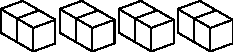
\includegraphics{P09-1}}\newline
Which of the following shapes cannot be made using these 4 blocks?}
{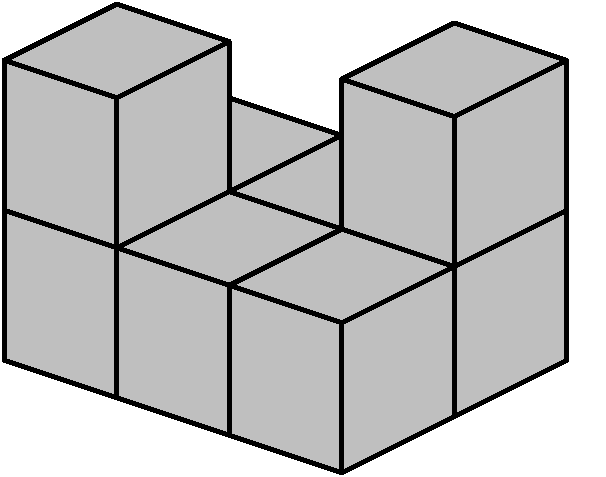
\includegraphics{P09-2}}{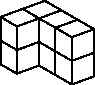
\includegraphics{P09-3}}{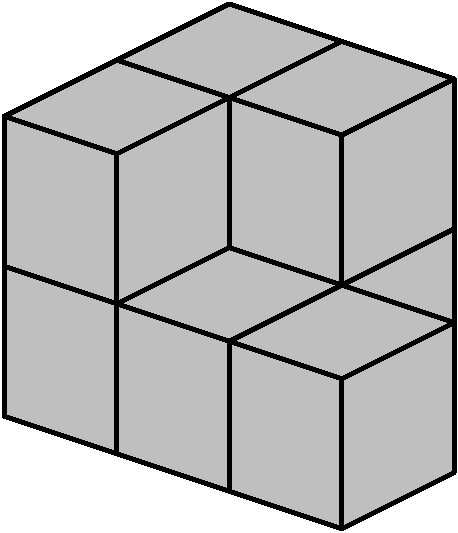
\includegraphics{P09-4}}{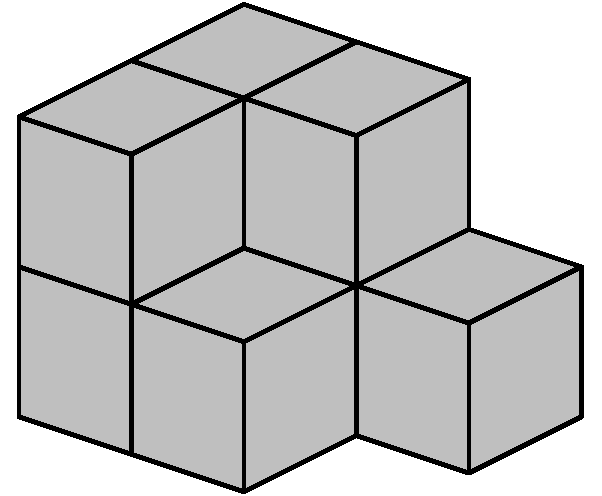
\includegraphics{P09-5}}{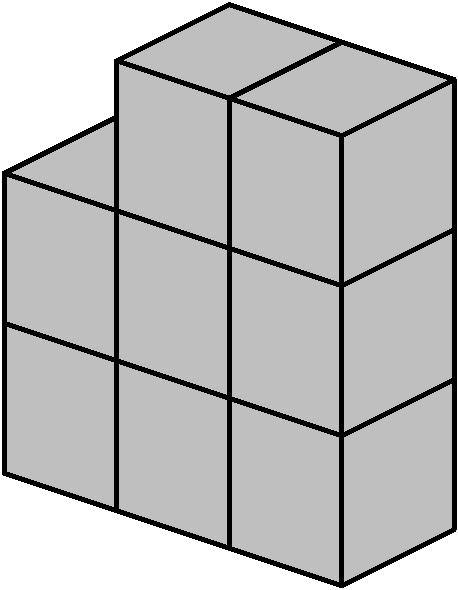
\includegraphics{P09-6}}
{D}{0}
{In figure D, it is not possible to put the 4 blocks together in such a way that the object could be created.}

\problemID{10}{20158}{Russia}%
\problemRating{P}{4}{A}%
\Problem{Chen has 5 baskets, each containing 4 toys.
\newline
\centerline{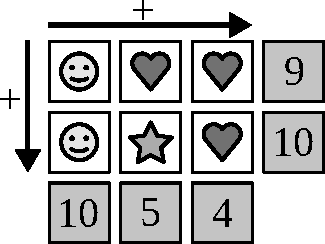
\includegraphics{P10-1}}
\newline
He dropped 4 of the baskets and the toys were mixed up.
\newline
\centerline{
\includegraphics{P10-2}}
\newline
Which basket did he not drop?}
{A}{B}{C}{D}{E}
{B}{0}
{There are 6 ducks in the mixed picture and 6 ducks in total across the 5 boxes. So all the boxes containing ducks were dropped, and the only one that was not dropped was (B).}

\problemID{11}{20159}{Indonesia}%
\problemRating{P}{4}{L}%
\Problem{In the following diagram, each shape represents a different value.
\newline
\centerline{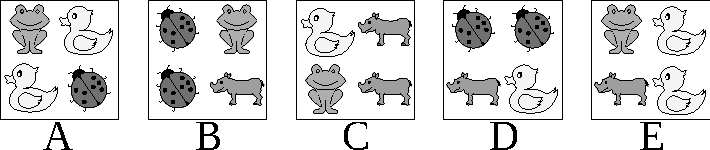
\includegraphics{P11-1}}
\newline
What is the value of 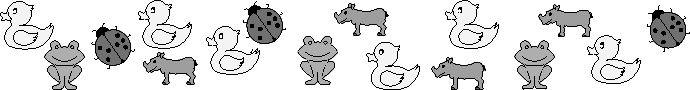
\includegraphics{P11-2}?}
{2}{3}{4}{5}{6}
{B}{0}
{As two hearts are 4, one heart is 2. 
As one heart and one star are 5, one star is $5 - 2 = 3$.}

\problemID{12}{20160}{Poland}%
\problemRating{P}{4}{N}%
\Problem{Catrina wants to walk through the maze so that she visits only rooms where the answer to the sum is 7.\newline
\centerline{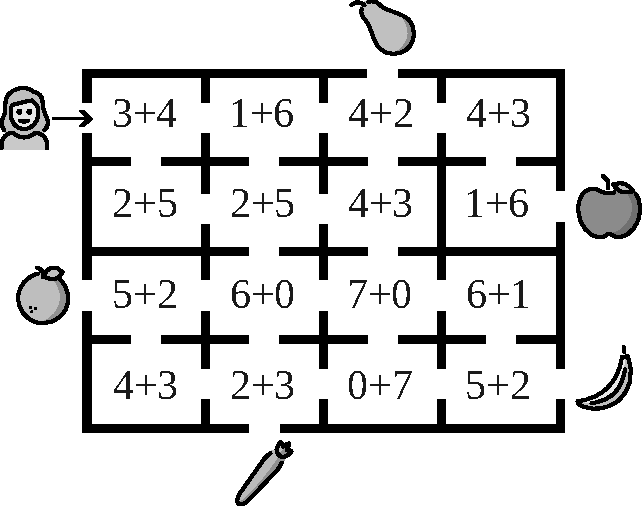
\includegraphics{P12-1}}
\newline
Which object can Catrina reach?}
{
\includegraphics[scale=0.8]{P12-2}}{
\includegraphics[scale=0.8]{P12-3}}{
\includegraphics[scale=0.8]{P12-4}}{
\includegraphics[scale=0.8]{P12-5}}{
\includegraphics[scale=0.8]{P12-6}}
{A}{0}
{First we find the sums. Then, we walk through the maze only visiting rooms with the sum 7. There is more than one possibility, but every possible way leads to the banana. One of the possibilities is shown below.\newline
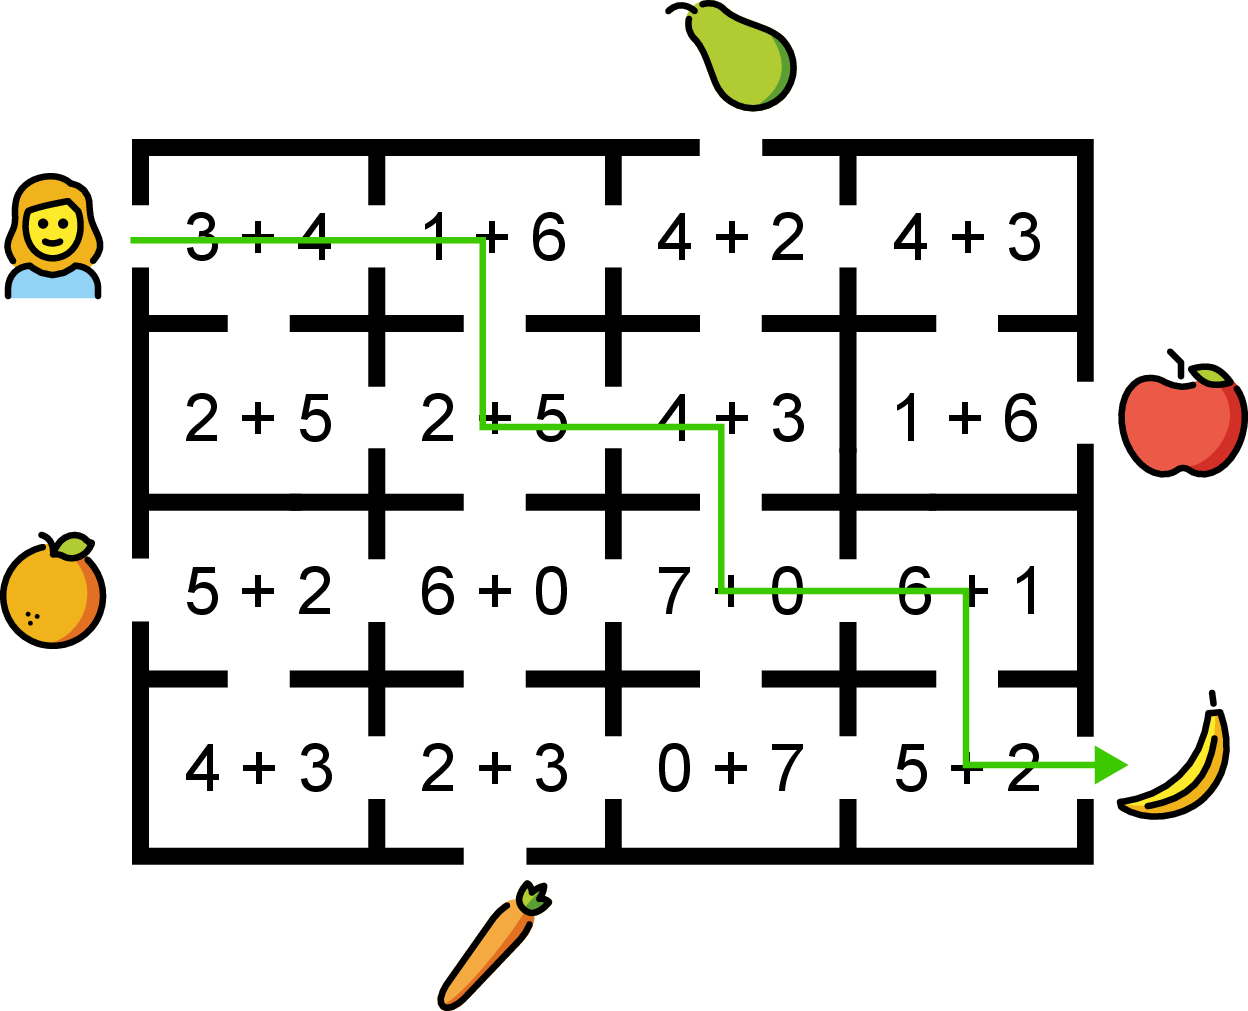
\includegraphics{P12-7}}

\problemID{13}{20161}{Finland}%
\problemRating{P}{4}{G}%
\Problem{A toy pony is inside a box that is 1 metre tall, 1 metre wide and 2 metres long. \newline
\centerline{
\includegraphics{P13-1}}
\newline
A ribbon goes around the box, as shown. The knot uses an extra 1 metre of ribbon.
How long is the ribbon in total?}
{9 metres}{11 metres}{13 metres}{15 metres}{17 metres}
{B}{0}
{We need $2 \times 2$ metres for the long sides; this is 4 metres. For the tall sides, we need $2 \times 1 = 2$ metres. For the wide side, we need $4 \times 1 = 4$ metres. For the knot, we need 1 metre. In total, the ribbon is $4 + 2 + 4 + 1 = 11$ metres long.}

\problemID{14}{20162}{Egypt}%
\problemRating{P}{4}{N}%
\Problem{The sum of the numbers in the triangle should be twice the sum of the numbers in the circle.
\newline
\centerline{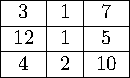
\includegraphics{P14-1}}
\newline
What number must replace the question mark?}
{3}{5}{8}{11}{16}
{D}{0}
{The sum of the numbers in the circle is 8. The sum of the numbers in the triangle must then be $2 \times 8 = 16$. So we must subtract 5 from 16 to get the answer. Doing that we have $16 - 5 = 11$.}

\problemID{15}{20163}{Catalonia}%
\problemRating{P}{4}{N}%
\Problem{A line of pictures is made by repeating this pattern of 5 pictures \includegraphics{P15-8} always in the same order.\newline
\centerline{\includegraphics{P15-9}}
\newline
Which picture is in the 27th position in the line?}
{\includegraphics{P15-10}}{\includegraphics{P15-11}}{\includegraphics{P15-12}}{\includegraphics{P15-13}}{\includegraphics{P15-14}}
{B}{0}
{The pattern repeats after every 5 pictures. So the 25th figure is a flame, the 26th is a sun, and the 27th is a ghost.

BW versions:
\includegraphics{P15-1}

\includegraphics{P15-2}

\includegraphics{P15-3}
\includegraphics{P15-4}
\includegraphics{P15-5}
\includegraphics{P15-6}
\includegraphics{P15-7}}

\problemID{16}{20164}{Turkey}%
\problemRating{P}{4}{N}%
\Problem{One of the numbers in the picture is equal to the sum of the numbers connected directly to it.  Which number is this?\newline
\centerline{\includegraphics{P16-1}}}
{3}{5}{7}{10}{12}
{C}{0}
{If you take the number 3, you can see connecting lines to the numbers 12, 1 and 1. $12 + 1 + 1 = 14$. 
14 is greater than 3. 
If we do this with all numbers, we see that 7 is the only number whose neighbours add up to the sum of $7 = 1 + 1 + 5$.\newline
\includegraphics{P16-2}}

\noindent\fbox{5 points}\bigskip

\problemID{17}{20165}{Greece}%
\problemRating{P}{5}{G}%
\Problem{Chiara has a transparent box containing 6 small cubes, as shown.
\newline
\centerline{\includegraphics{P17-1}}
\newline
What does Chiara see if she looks at the box from above?}
{\includegraphics{P17-2}}{\includegraphics{P17-3}}{\includegraphics{P17-4}}{\includegraphics{P17-5}}{\includegraphics{P17-6}}
{E}{0}
{If we look at the object from above, we see three cubes in the upper left corner. At the bottom right is a cube that we can see through the transparent glass. This cube can also be seen from above.

\includegraphics{P17-7}}

\problemID{18}{20166}{Greece}%
\problemRating{P}{5}{N}%
\Problem{Esteban wants to pick two numbers from the board and add them together.\newline
\centerline{\includegraphics{P18-1}}\newline
How many different results could Esteban get?}
{5}{6}{7}{8}{10}
{C}{0}
{The smallest possible answer he can get is $1 + 2 = 3$ and the largest is $4 + 5 = 9$. All the other numbers he can get are in between those two. In other words, all possible numbers he can get are definitely among 3, 4, 5, 6, 7, 8, 9. In fact he can get all these numbers as seen from the calculations $1 + 2 = 3$; $1 + 3 = 4$; $1 + 4 = 5$; $2 + 4 = 6$; $3 + 4 = 7$; $3 + 5 = 8$; $4 + 5 = 9$.  Counting them we see that he can get 7 possible different results.

=== alternative solution ===
Writing out the possible sums in order:
$1 + 2 = 3$;
$1 + 3 = 4$;
$1 + 4 = 5$;
$1 + 5 = 6$;
$2 + 3 = 5$;
$2 + 4 = 6$;
$2 + 5 = 7$;
$3 + 4 = 7$;
$3 + 5 = 8$;
$4 + 5 = 9$.
We get 10 sums overall but 3 of them have equal answers, so we can get 7 different answers.}

\problemID{19}{20167}{Ecuador}%
\problemRating{P}{5}{L}%
\Problem{Which two pieces can be used to complete the grid without overlapping?
\newline
\centerline{\includegraphics{P19-1}}}
{1 and 2}{1 and 3}{3 and 4}{2 and 4}{2 and 3}
{E}{0}
{\includegraphics{P19-2}\newline
So we need piece 2 and piece 3 to complete the grid. Our solution is E.}

\problemID{20}{20168}{Russia}%
\problemRating{P}{5}{L}%
\Problem{Ali, Bella, Che and Dimitry each have 3 shapes. Each child has exactly one shape in common with every other child.
\newline
\centerline{\includegraphics{P20-1}}
\newline
Which shapes does Dimitry have?}
{\includegraphics{P20-2}}{\includegraphics{P20-3}}{\includegraphics{P20-4}}{\includegraphics{P20-5}}{\includegraphics{P20-6}}
{D}{1}
{Ali and Bella both have a square. Bella and Che both have a star. 
Ali and Che both have a triangle. So Dimitry must have a circle like Ali, a heart like Bella, and a square like Che.

\includegraphics{P20-7}}

\problemID{21}{20169}{Poland}%
\problemRating{P}{5}{N}%
\Problem{Zoran builds towers from three types of blocks. The heights of three of them are shown in the picture.
\newline
\centerline{\includegraphics{P21-1}}
\newline
What is the height of the fourth tower?}
{\(12\)}{\(13\)}{\(14\)}{\(16\)}{\(17\)}
{A}{0}
{\includegraphics{P21-2}
If we compare the first and third tower, we find that the triangle is 5 units high ($20 - 15 = 5$). Now, if we compare the second and third tower, we find that the rectangle is 7 units high. ($20 - 13 = 7$).
The tower made from a rectangle and a triangle is therefore $12 = 7 + 5$ units high.}

\NSidePictureEPS[scale=1.2]{P22-1}{\problemID{22}{20170}{Catalonia}%
\problemRating{P}{5}{N}%
\Problem{Zara wants to move through the grid from $A$ to $B$. She can only move to the right or upwards. Each time she visits a grey box, she has to pay 1 euro. Each time she visits a white box, she has to pay 2 euros. How much would she pay for the cheapest path?}
{11 euros}{12 euros}{13 euros}{15 euros}{16 euros}
{C}{1}
{Zara has to pay more for a white box than for a grey box. So she has to go through as few white boxes as possible. To get from A to B, she has to take 8 steps: 5 to the right and 3 up. We can find some paths that go through 5 white boxes, but no path that goes through 4 white boxes. So the cost of the cheapest way is $5 \times 2 + 3 \times 1 = 13$ euros.}}

\problemID{23}{20171}{Brazil}%
\problemRating{P}{5}{N}%
\Problem{Julia has a list of problems to finish during May. She starts on the 1st of May.\newline
\centerline{\includegraphics[scale=0.25]{P23-1}}\newline
If she solves exactly 2 problems each day, she will finish the task on a Sunday. If she solves exactly 3 problems each day, she will finish the task on a Wednesday. How many problems are on the list?}
{6}{12}{18}{24}{30}
{D}{0}
{If Julia solves 2 problems per day and finishes on a Sunday, then there must be either 10, 24, 38 or 52 problems on the list. If Julia solves 3 problems per day and finishes on a Wednesday, then there must be either 3, 24, 45, 66 or 87 problems. The only number that these two lists have in common is 24.}

\problemID{24}{20172}{Belarus}%
\problemRating{P}{5}{L}%
\Problem{Andrew was throwing darts at a target. He started with 10 darts and got 2 new darts each time he hit the target. In total, Andrew threw 20 darts and then had no darts left. How many times did Andrew hit the target?}
{$4$}{$5$}{$6$}{$8$}{$10$}
{B}{0}
{For each hit, Andrew gets two more darts. 
He threw 20 in total, and so must have got $20-10=10$ more than he had at the beginning. He would have got $10$ extra darts by hitting the target $10\div 2=5$ times.}


\end{document}